\section{Outreach}
As a team, de.evolution believes that robotics is more than just the engineering. Our first year as a team we saw that the other FTC team at our school, Domo Arigato, was entirely seniors and we were sad that it was going to disappear. This inspired us to try and spread robotics to the younger students and have people involved to keep robotics teams going and to propogate the message of FIRST throughout our community. We have started a robotics class at our high school which has turned into the team Domo Arigato. Due to the popularity of the class a second class, and subsequently an FTC team, has been started. Both the Robo Ravens and Domo Arigato, along with our own team, de.evolution, work hard to start a robotics and engineering culture at our school. The section will be structured as follows, we will begin by listing our community outreach and will in the subsequent subsections go into further detail about some of the more important work we do

\subsection{Community Outreach}
As a team, de.evolution has tried to do a lot to help spread the ideas of FIRST, robotics and engineering. The following is an extensive list of some of the community outreach that we have done:

\begin{enumerate}
\item Robotics demos to elementary school students at Solana Pacific Elementary, Del Mar Heights Elementary, Rancho Santa Fe Elementary
\item PTC World demo in June 2013
\item Mentoring of the three Islamic School of San Diego FLL teams 
\item Sister team of the San Dieguito Academy FTC teams Paradox Squared and Paradox Cubed
\item Demo for school board \& superintendent – sponsored building/engineering production district-wide with bond measure
\item Hosted Robotics Week at CCA in coordination with Domo Arigato
\item Publication in newspapers \& press releases about stem/robotics
\item Publication in school's magazines
\item Over 20\% of school has become involved with the FIRST robotics programs after the inception of our team
\item Inspired the FIRST robotics classes
\item Incorporating art and conservatory at CCA with the robotics program
\item Incorporating the humanities conservatory at CCA with the robotics teams
\item Working with TEDxYouth@SanDiego to spread robotics to the students in San Diego
\item Hosted small scrimmages at home
\item Hosting fundraisers at Souplantation for FIRST robotics
\item Attended and presented at Rotary meetings to show our community the influence of robotics
\end{enumerate}

\subsection{Helping other teams online}
As the majority of the members on our team are also on the FRC team \underline{The Aluminum Narwhals} we realize that having online support is one of the best ways to debug and learn about robotics. Chief Delphi, one of the prominent places for online FIRST discussion, is very popular among FRC teams. However, FTC teams do not have nearly as much online support as they may need or like. As a team we have shifted a lot of our focus to helping teams online. We have open-sourced all of our code and have created code tutorials to help out many other teams. In specific we have helped teams in the following ways:

\subsubsection{Syntax Error code optimization assistance}

At a San Diego regional qualification competition, we entered a discussion with team 6077, Syntax Error, about code optimization. We were sharing our varied tricks which were used in code, and through discussion, it became clear that there were a couple points they were particularly interested in implementing. We passed them some contact information, and later received an email from them:

\begin{lstlisting}
Hey Noah,

We're interested in optimizing the speed of our teleop code, and I know you had mentioned at the tournament that you guys XOR-ed the joystick values to determine when the values had changed--allowing you to skip checks when things weren't changing. Could you please go into more depth as to how you achieved this? Did you directly modify joystickdriver.c? Which values should we be XOR-ing exactly?

Thanks,
-Collin 
\end{lstlisting}

We wrote out a document generally detailing the approaches we took when optimizing our teleoperated code. My response was the following PDF file:

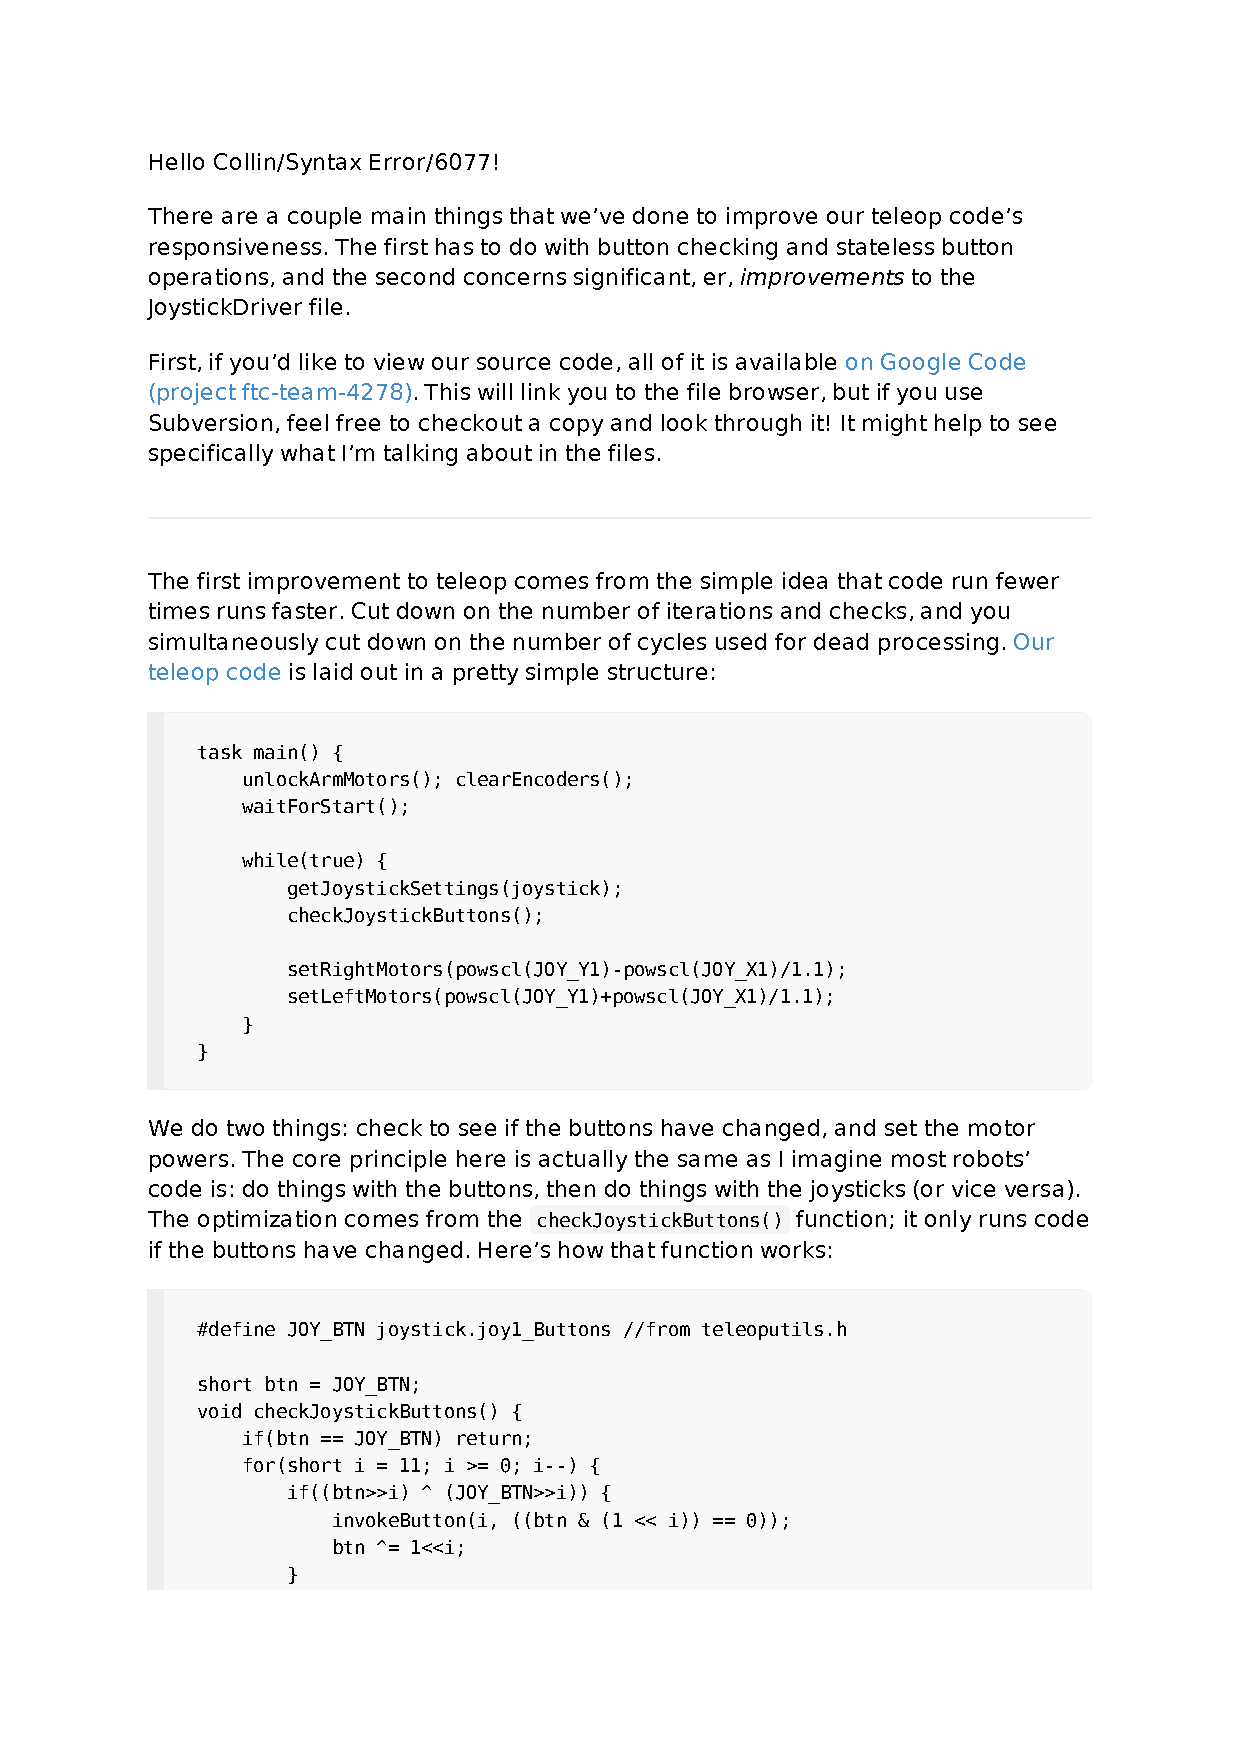
\includepdf[pages={1-2}]{SyntaxError.pdf}

The aim was to create an easy-to-follow guide for someone with experience to optimize the teleoperated program. To our enjoyment, they reported significant increases in response time on their controller.

\subsubsection{Reddit}

\subsection{Mentoring of FLL teams}
Our team aided the Islamic School of San Diego's FLL Teams during their rookie years by mentoring the young kids on robotics and the engineering design process in general. Our students voluntarily watched over the excited and energetic children, assisted in teaching them key concepts, and created useful PowerPoint presentations that were presented to further educate the FLL teams.

In each meeting, the FLL teams was taught a concept and then given time to build something from LEGOs using their newfound knowledge. Since our de.evolution volunteers were there, the FLL leader could split the team into small groups with a mentor or leader helping each group. Another advantage of having an FTC mentor available was that the volunteer could lead the team while the leader temporarily prepared the next lesson or dealt with other essential tasks. It relieved the leader of FLL and kept everything running smoothly.

The lessons taught the eager and energetic students about what causes earthquakes and the destruction that they inflict. This understanding supported the kids in cooperatively creating ideas for a machine to aid anyone who recently experienced a devastating disaster. The mentors also educated the group about the engineering design process to assist them in efficiently building a better solution when they were ready to begin fabrication of their product.

We found that mentoring FLL teams has not only allowed us to teach the students a lot about robotics, but we gained valuable experiences by doing so.
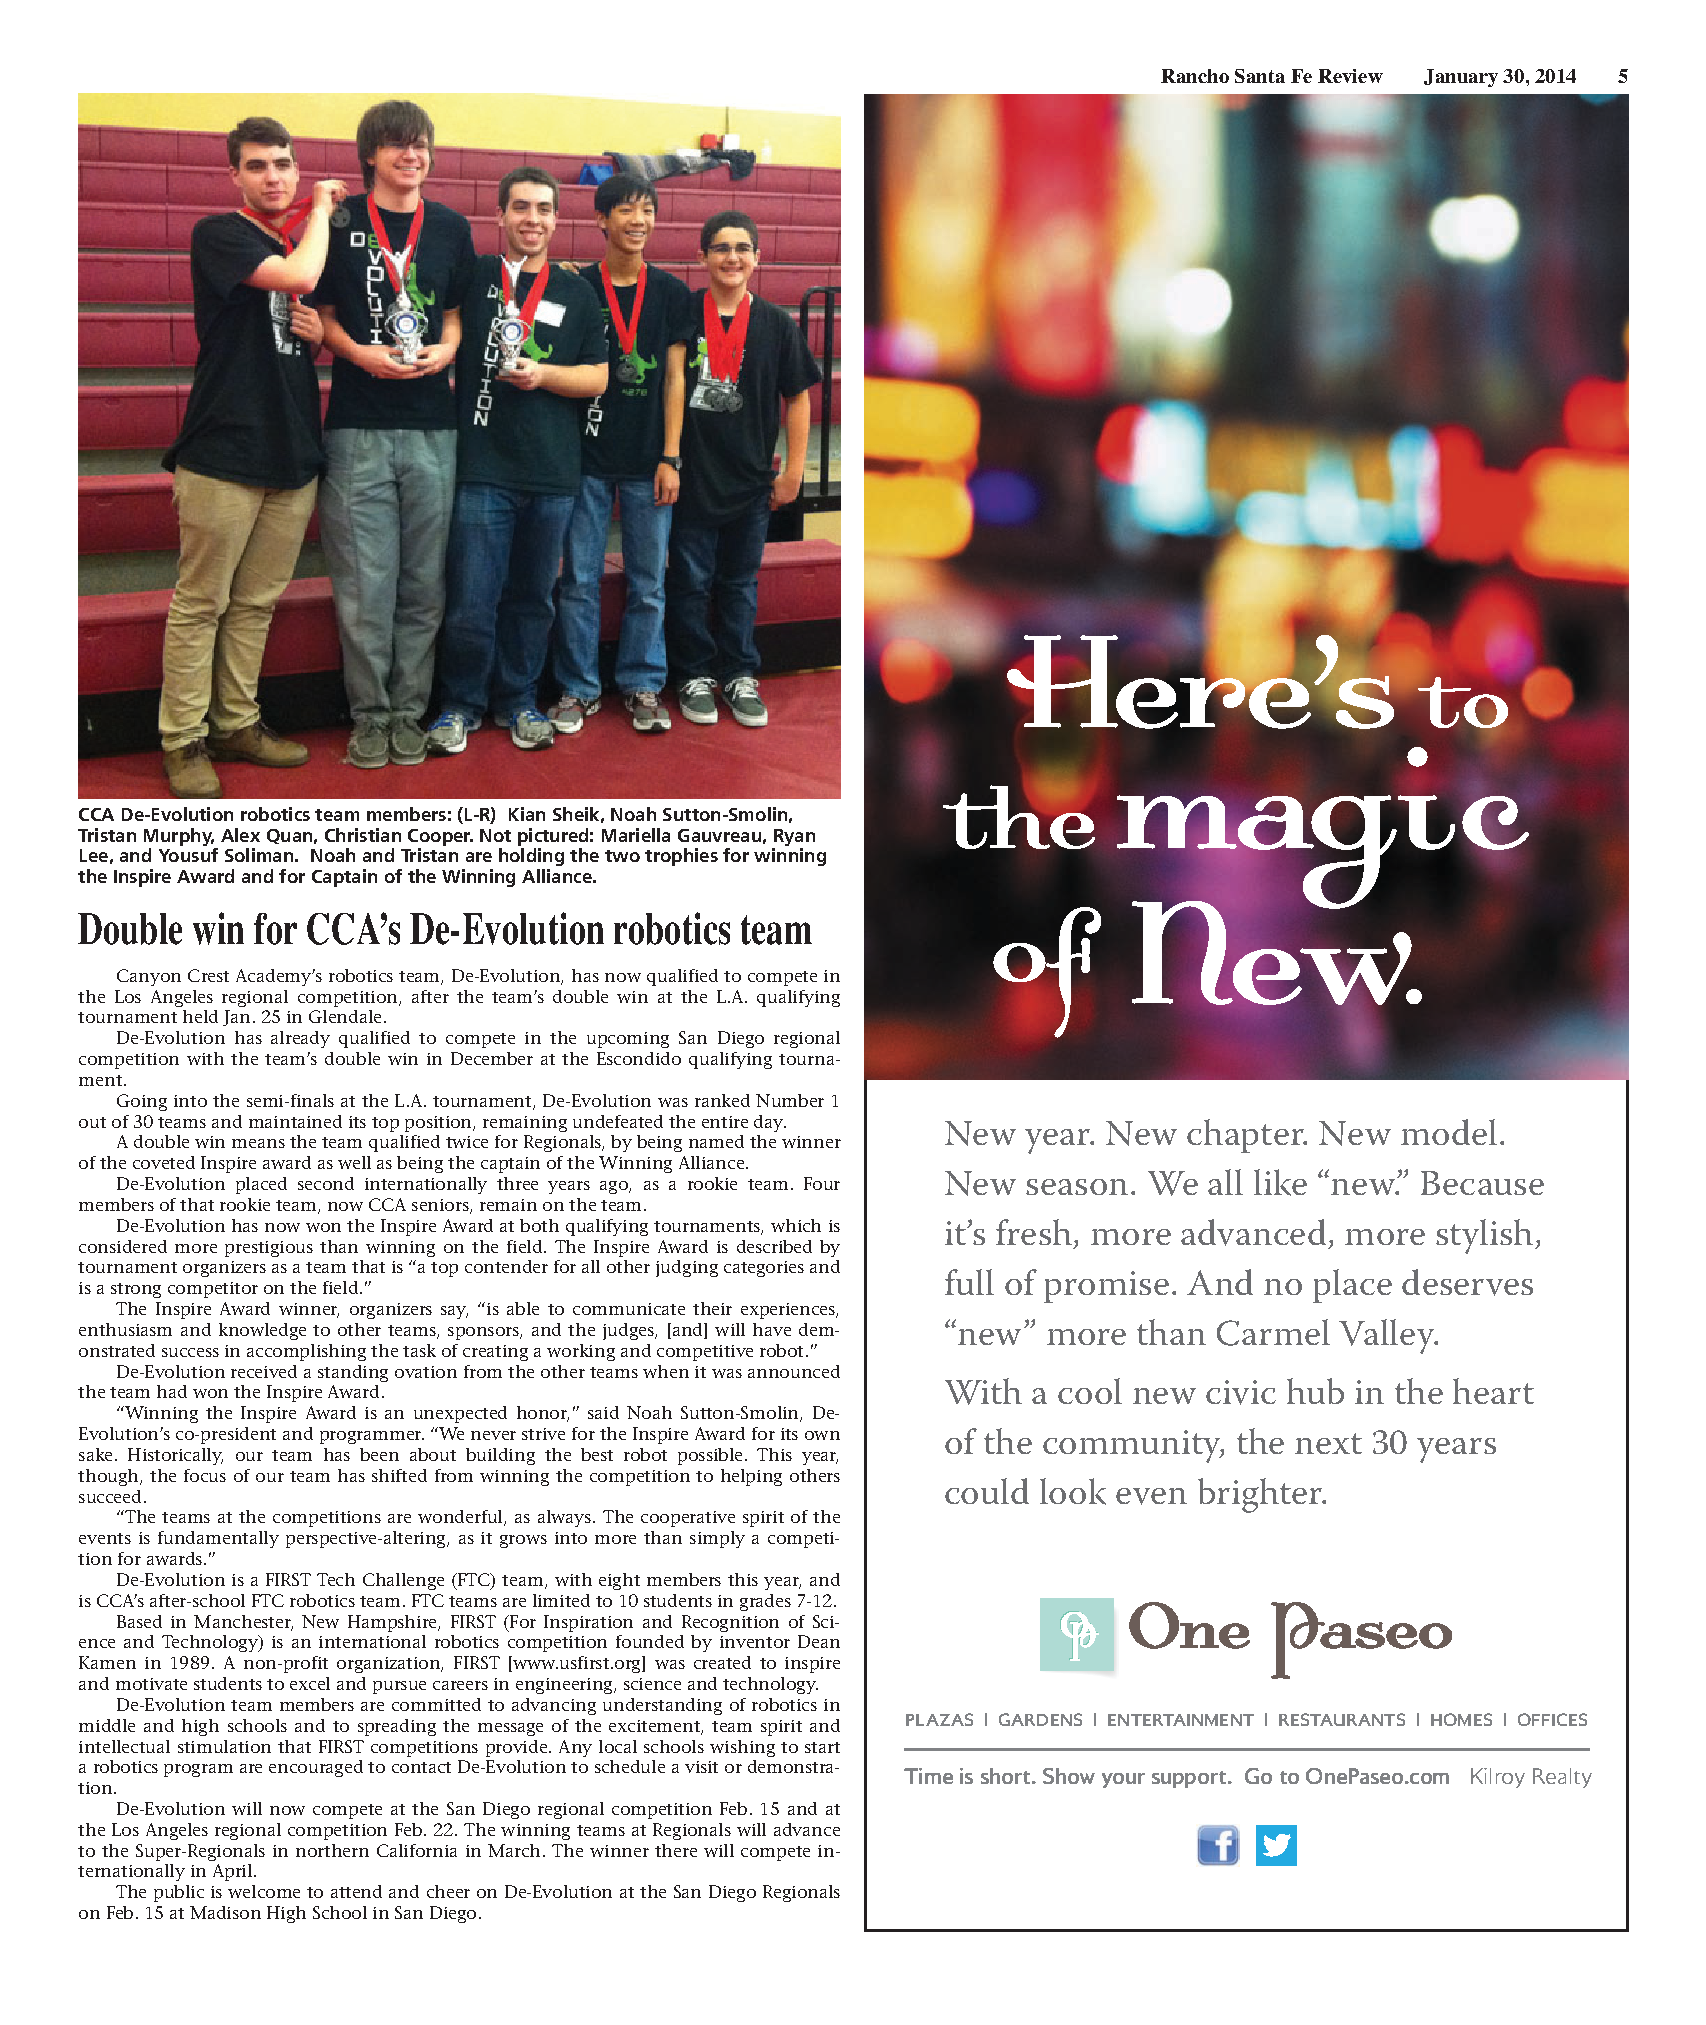
\includepdf[pages={-}]{DoubleWinNewspaper.pdf}

\subsection{Meeting with the SDUHSD Disctrict Office}

A while back, we met with the San Diego Union High School District (SDUHSD) district office to present the FIRST Tech Challenge program. It was a significant demonstration, as our ultimate goal was to inspire further funding for robotics in regional high schools.

Our efforts paid off. Recently, Proposition AA, an educational bond bill, was passed in the San Diego area. This included significant funding for the construction of a robotics building at our host high school, Canyon Crest Academy. We have already brought approximately 15 to 20\% of the high school population through some form of FIRST's programs, and this will hopefully expand both the educational capacity and general awareness of FIRST among the high school students.